\documentclass[10pt,aspectratio=169]{beamer}
\usepackage{udec-slides}
\slide{3}{Ley de Gauss}

\begin{document}
\primeraDiapo

\begin{frame}{Ley de Gauss}{Medios Dieléctricos}
    \begin{boxTeoria}{Ley de Gauss Generalizada}
        \begin{columns}[T] % [T] alinea al tope de las columnas

            % Primera Columna: Ecuaciones
            \begin{column}{0.48\textwidth}
                El flujo de $\vec{D}$ es igual a la carga libre encerrada:
                \begin{equation*}
                    \oint_S \vec{D} \cdot \, d\vec{A} = Q_{f, \text{enc}}
                \end{equation*}
                En medios lineales: $\vec{D} = \epsilon \vec{E}$
            \end{column}

            % Segunda Columna: Definiciones
            \begin{column}{0.48\textwidth}
                Donde:
                \begin{itemize}
                    \item $\vec{D}$: Desplazamiento eléctrico.
                    \item $\epsilon$: Permitividad del medio ($\epsilon_1, \epsilon_2, \epsilon_0$).
                    \item $Q_{f, \text{enc}}$: Carga libre (no de polarización).
                \end{itemize}
            \end{column}

        \end{columns}
    \end{boxTeoria}
    \small \textbf{Nota:} Como se ve en la figura anterior, el valor de $\epsilon$ cambia según la región, afectando directamente la magnitud de $\vec{E}$.
\end{frame}

\begin{frame}{Problema 1}
    \begin{columns}[c]

        \begin{column}{0.55\textwidth}
            Considere una esfera de radio $R_2$ compuesta por dos materiales dieléctricos con carga distribuida uniformemente:

            \begin{itemize}
                \item \textbf{Región I} ($0 < r < R_1$): \\ Permitividad $\epsilon_1$, densidad $\rho_1$.
                \item \textbf{Región II} ($R_1 < r < R_2$): \\ Permitividad $\epsilon_2$, densidad $\rho_2$.
                \item \textbf{Región III} ($r > R_2$): \\ Vacío ($\epsilon_0$).
            \end{itemize}

            Determine la expresión para la magnitud del campo eléctrico $E(r)$ en cada una de las tres regiones.
        \end{column}

        \begin{column}{0.45\textwidth}
            \centering
            \begin{minipage}{0.6\textwidth}
                \centering
                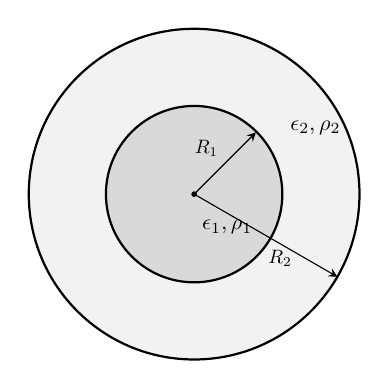
\begin{tikzpicture}[scale=1.4]
                    \draw[fill=gray!10, thick] (0,0) circle (1.5);
                    \draw[fill=gray!30, thick] (0,0) circle (0.8);
                    \draw[fill=black] (0,0) circle (0.02);

                    % Usamos "stealth-" y "-stealth" en lugar de flechas con ">"
                    \draw[-stealth] (0,0) -- (0.56, 0.56) node[midway, above left, scale=0.7] {$R_1$};
                    \draw[-stealth] (0,0) -- (1.3, -0.75) node[pos=0.6, below, scale=0.7] {$R_2$};

                    \node[scale=0.8] at (0.3, -0.3) {$\epsilon_1, \rho_1$};
                    \node[scale=0.8] at (1.1, 0.6) {$\epsilon_2, \rho_2$};
                \end{tikzpicture}
            \end{minipage}
        \end{column}

    \end{columns}
\end{frame}

\begin{frame}{Problema 2}
    Considere un cable recto, muy delgado e infinitamente largo, que posee una densidad lineal de carga $\lambda$ (uniforme en toda su longitud).

    Obtenga una expresión para la magnitud de campo eléctrico a una distancia $r$ del cable.

    \begin{figure}[H]
        \centering
        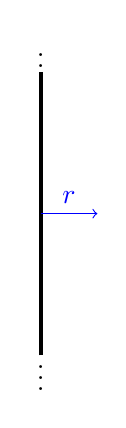
\begin{tikzpicture}[scale=0.6]
            % Línea infinita de carga (el cable) con puntos suspensivos
            \draw[ultra thick] (0, -3) -- (0, 3);
            \node at (0, 3.3) {$\vdots$};
            \node at (0, -3.3) {$\vdots$};

            % Etiqueta del radio gaussiano r
            \draw[->, blue] (0,0) -- (1.2, 0) node[midway, above] {$r$};
        \end{tikzpicture}
    \end{figure}
\end{frame}

\begin{frame}{Problema 3}
    Se tiene una placa plana infinita de material aislante, la cual posee una densidad superficial de carga $\sigma$ uniforme.

    Encuentre la magnitud del campo eléctrico $E$ a una distancia $z$ de la placa.

    \begin{figure}[H]
        \centering
        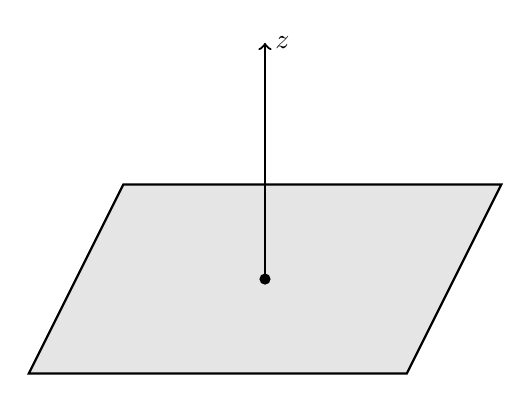
\begin{tikzpicture}[scale=1.2]
            % Plano infinito en z=0 (acostado en perspectiva)
            \draw[fill=gray!20, thick] (-2.5, -1) -- (1.5, -1) -- (2.5, 1) -- (-1.5, 1) -- cycle;

            % Parte saliendo hacia arriba
            \draw[->, thick] (0, 0) -- (0, 2.5) node[right] {$z$};

            % Punto de origen en el plano
            \filldraw[black] (0,0) circle (1.5pt);
        \end{tikzpicture}
    \end{figure}
\end{frame}


\end{document}